 \documentclass[t, xcolor=table]{beamer}
%\documentclass[c]{beamer}
\listfiles

\newcommand{\putat}[3]{\begin{picture}(0,0)(0,0)\put(#1,#2){#3}\end{picture}}
\newcommand*{\xMin}{-6}%
\newcommand*{\xMax}{6}%
\newcommand*{\yMin}{-6}%
\newcommand*{\yMax}{5}%
\setbeamertemplate{section in toc}[sections numbered]
\setbeamertemplate{subsection in toc}[subsections numbered]

\defbeamertemplate{subsubsection in toc}{subsubsections numbered}
{\leavevmode\leftskip=3em%
 \rlap{\hskip-3em\inserttocsectionnumber.\inserttocsubsectionnumber.\inserttocsubsubsectionnumber}%
 \inserttocsubsubsection\par}

\definecolor{kit-green}{RGB}{0, 150, 130}
\definecolor{kit-blue}{RGB}{70, 100, 170}
\definecolor{kit-lightgreen}{RGB}{140, 182, 60}
\definecolor{kit-orange}{RGB}{223, 155, 27}
\definecolor{kit-red}{RGB}{162, 34, 35}

\setbeamercolor{alerted text}{fg=kit-green}
% Darkened version: {fg=kit-green!80!black}

\mode<presentation>
{
  \usetheme[usefoot,english,cmyk,titlepage0]{KIT}
% \usetheme[usefoot]{KIT}
% \usetheme{KIT}

%%  \usefonttheme{structurebold}

  \setbeamercovered{transparent}

  %\setbeamertemplate{enumerate items}[circle]
  \setbeamertemplate{enumerate items}[ball]
%  \setbeamerfont{section in toc}{color=black}
  \setbeamercolor{section number projected}{bg=black,fg=yellow}
  \setbeamertemplate{subsection in toc}[subsubsections numbered]

}
\usepackage{tabularx}
\usepackage{pdfpages}
\usepackage{caption}
\usepackage{pbox}
\usepackage{multirow}
\usepackage{babel}
\usepackage{feynmp-auto}
\usetikzlibrary{calc}
\date{2018-07-09}
%\DateText

\newlength{\Ku}
\setlength{\Ku}{1.43375pt}

\usepackage[latin1]{inputenc}
\usepackage[TS1,T1]{fontenc}
\usepackage{array}
\usepackage{multicol}
\usepackage[makeroom]{cancel}
\usepackage{subfigure}
\usepackage{xspace}
%\usenavigationsymbols
%\usenavigationsymbols[sfHhdb]
%\usenavigationsymbols[sfhHb]
\newcommand{\verysmall}{\fontsize{6pt}{8.6pt}\selectfont}
\usepackage{siunitx}


\DeclareSIUnit\clight{\ensuremath{c}}
\DeclareSIUnit[per-mode=symbol]\GeVc{\GeV\per\clight}
\DeclareSIUnit[per-mode=symbol]\GeVcc{\GeV\per\clight\squared}
\DeclareSIUnit\fb{\femto\barn}
\DeclareSIUnit\invfb{\per\femto\barn}

\newenvironment<>{neutralblock}[1]{%
  \begin{actionenv}#2%
      \def\insertblocktitle{#1}%
      \par%
      \mode<presentation>{%
        \setbeamercolor{block title}{fg=white,bg=gray!70!black}
       \setbeamercolor{block body}{fg=black,bg=gray!50}
       \setbeamercolor{itemize item}{fg=white}
       \setbeamertemplate{itemize item}[triangle]
     }%
      \usebeamertemplate{block begin}}
    {\par\usebeamertemplate{block end}\end{actionenv}}

\newenvironment<>{redblock}[1]{%
  \begin{actionenv}#2%
      \def\insertblocktitle{#1}%
      \par%
      \mode<presentation>{%
        \setbeamercolor{block title}{fg=white,bg=red!70!black}
       \setbeamercolor{block body}{fg=black,bg=red!30}
       \setbeamercolor{itemize item}{fg=white}
       \setbeamertemplate{itemize item}[triangle]
     }%
      \usebeamertemplate{block begin}}
    {\par\usebeamertemplate{block end}\end{actionenv}}

\newenvironment<>{blueblock}[1]{%
  \begin{actionenv}#2%
      \def\insertblocktitle{#1}%
      \par%
      \mode<presentation>{%
        \setbeamercolor{block title}{fg=white,bg=blue!70!black}
       \setbeamercolor{block body}{fg=black,bg=blue!30!white!80}
       \setbeamercolor{itemize item}{fg=white}
       \setbeamertemplate{itemize item}[triangle]
     }%
      \usebeamertemplate{block begin}}
    {\par\usebeamertemplate{block end}\end{actionenv}}

\newenvironment<>{greenblock}[1]{%
  \begin{actionenv}#2%
      \def\insertblocktitle{#1}%
      \par%
      \mode<presentation>{%
        \setbeamercolor{block title}{fg=white,bg=green!70!black}
       \setbeamercolor{block body}{fg=black,bg=green!50}
       \setbeamercolor{itemize item}{fg=white}
       \setbeamertemplate{itemize item}[triangle]
     }%
      \usebeamertemplate{block begin}}
    {\par\usebeamertemplate{block end}\end{actionenv}}

\title[]{Modeling and Simulation of Load Balancing Strategies for Computing in High Energy Physics}
\subtitle{Karlsruhe Institute of Technology (KIT)}

\subtitle[Ren\'e Caspart]{\underline{\smash{Ren\'e Caspart}}, Patrick Firnkes, Manuel Giffels, Anne Koziolek, G\"unter Quast, Ralf Reussner}

\AuthorTitleSep{\relax}

\institute[]{KARLSRUHE INSTITUTE OF TECHNOLOGY (KIT)}

\TitleImage[width=\titleimagewd]{Bilder/KIT-Titel}

\newlength{\tmplen}

\begin{document}


%%%%%%%%%%%%%%%%%%%%%%%%%%%%%%%%%%%%%%%%%%%%%%%%%%%%%%%%%%%%%%%%%%%%%%%%%%%%%%%%%%%%%%%%%%%%%%%%%%%%%%%%%%%%%%%%%%%%%%%%%%%%%%%%%%%%%%%%%%%%%%
\begin{frame}
  \maketitle
\end{frame}

%%%%%%%%%%%%%%%%%%%%%%%%%%%%%%%%%%%%%%%%%%%%%%%%%%%%%%%%%%%%%%%%%%%%%%%%%%%%%%%%%%%%%%%%%%%%%%%%%%%%%%%%%%%%%%%%%%%%%%%%%%%%%%%%%%%%%%%%%%%%%%
\AtBeginSection[]
{
\begin{frame}
\frametitle{Table of Contents}
\tableofcontents[currentsection,%currentsubsection, 
%    hideothersubsections, 
    sectionstyle=show/shaded,
    subsectionstyle=hide/hide,
]
\end{frame}
}

%%%%%%%%%%%%%%%%%%%%%%%%%%%%%%%%%%%%%%%%%%%%%%%%%%%%%%%%%%%%%%%%%%%%%%%%%%%%%%%%%%%%%%%%%%%%%%%%%%%%%%%%%%%%%%%%%%%%%%%%%%%%%%%%%%%%%%%%%%%%%%

\section*{Motivation}
\begin{frame}
    \frametitle{Motivation}
    \begin{columns}
        \begin{column}{0.45\textwidth}
            \begin{itemize}
                \item Flat computing budget model does not cover future needs for computing resources
                \item Need to find ways to deal with this lack of resources
                \begin{itemize}
                    \item Addition of non-HEP specific resources
                    \item Improvement of used algorithms and software
                    \item Improvement of utilization of computing centers
                \end{itemize}
            \end{itemize}
        \end{column}
        \hfill
        \begin{column}{0.5\textwidth}
            \begin{center}
                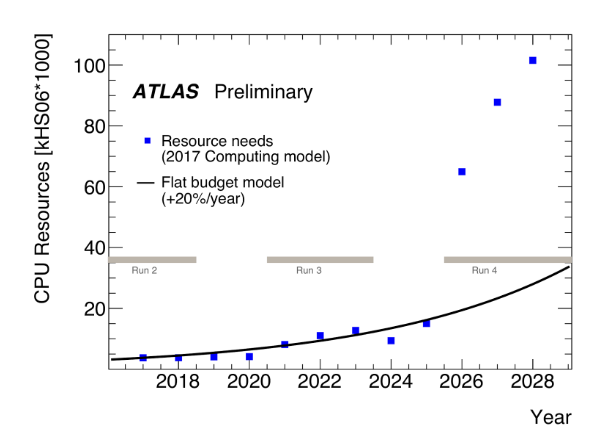
\includegraphics[width=\textwidth]{Bilder/CPU_resources_budget}
                \hspace{-2cm}
                \tiny{https://arxiv.org/abs/1712.06982}
                %\includegraphics[width=\textwidth]{Images/cpuefficiency_T1s_allactivities}
            \end{center}
        \end{column}
    \end{columns}
\end{frame}

\begin{frame}
    \frametitle{Current Status}
    \begin{columns}
        \begin{column}{0.45\textwidth}
            \begin{itemize}
                \item Efficiency of utilization of grid sites not optimal
                \item We want to address two effects 
                \begin{itemize}
                    \item Impact on efficiency due to site limitations (e.g. network or storage bandwidth)
                    \item Impact on efficiency due to scheduling overhead
                \end{itemize}
            \end{itemize}
        \end{column}
        \hfill
        \begin{column}{0.5\textwidth}
            \begin{center}
                \vspace{-4ex}
                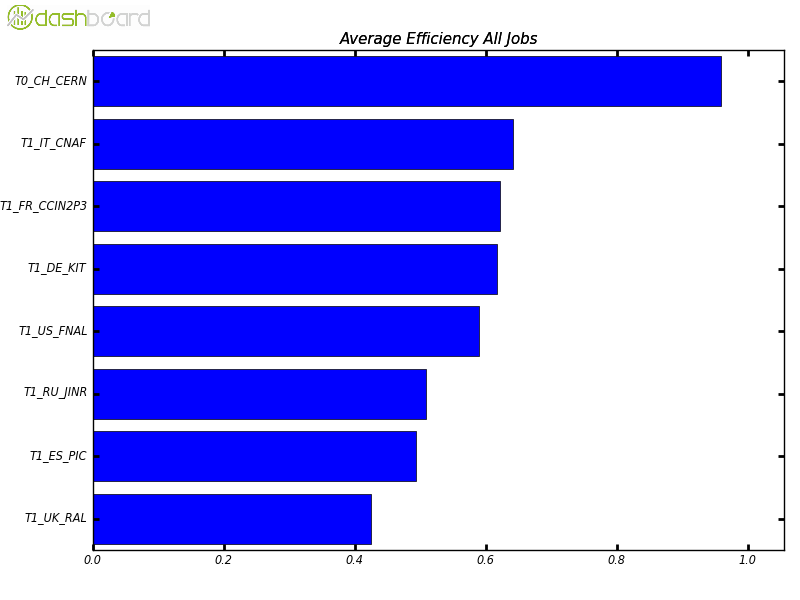
\includegraphics[width=\textwidth]{Bilder/Eff_T0_T1}
                \vspace{2ex}
                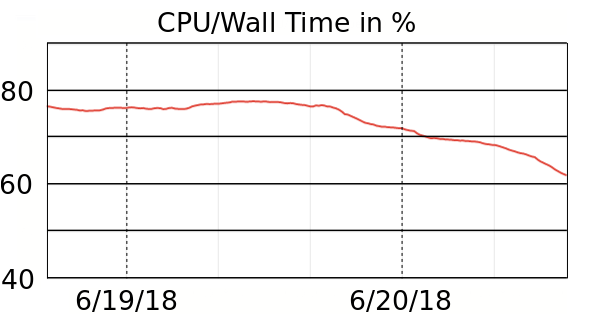
\includegraphics[width=\textwidth]{Bilder/CPU_eff_gridKa}
            \end{center}
        \end{column}
    \end{columns}
\end{frame}


\section*{Concept \& Proof of Work}
\begin{frame}
\frametitle{Concept \& Proof of Work}
\begin{columns}
	\begin{column}{0.45\textwidth}
		\begin{exampleblock}{Concept}
		\begin{itemize}
			\setlength\itemsep{1em}
			\item Create simulation for WLCG to optimize resource usage
			\begin{itemize}
				\item Evaluate load balancing strategies
				\item Evaluate grid infrastructure improvements
				\item Evaluate scheduling decisions
			\end{itemize}
		\end{itemize}
	\end{exampleblock}
	\end{column}
	\hfill
	\begin{column}{0.45\textwidth}
		\begin{exampleblock}{Proof of work}
			\begin{itemize}
			\item Created simulation for CMS computing jobs at GridKa
			\item Used Palladio Simulator as foundation
			\item Implemented automatic parameter extraction and model creation
			\item Validated first results
			\end{itemize}
	\end{exampleblock}
	\end{column}
\end{columns}
\end{frame}

\note[itemize]{
	\item evaluate to find best from a given set
}

\section*{Palladio Simulator}
\begin{frame}
\frametitle{Palladio Simulator}
\begin{columns}
	\begin{column}{0.47\textwidth}
		\begin{itemize}
					\setlength\itemsep{1em}
			\item Enables performance predictions for design decisions
			\item Event-based model driven software architecture simulator
			\item Model on abstract level: Express resource needs of jobs as statistical distribution
			\item Extended for simulation of Cloud Computing/HPC
			\begin{itemize}
				\item Architectural Templates: Model large systems efficiently
				\item SimuLizar: Simulate self adapting systems
			\end{itemize}
		\end{itemize}
	\end{column}
	\hfill
	\begin{column}{0.5\textwidth}
		\begin{itemize}
			\item Successfully used for optimizing cloud infrastructure as part of the CACTOS project
		\end{itemize}
			\begin{center}
				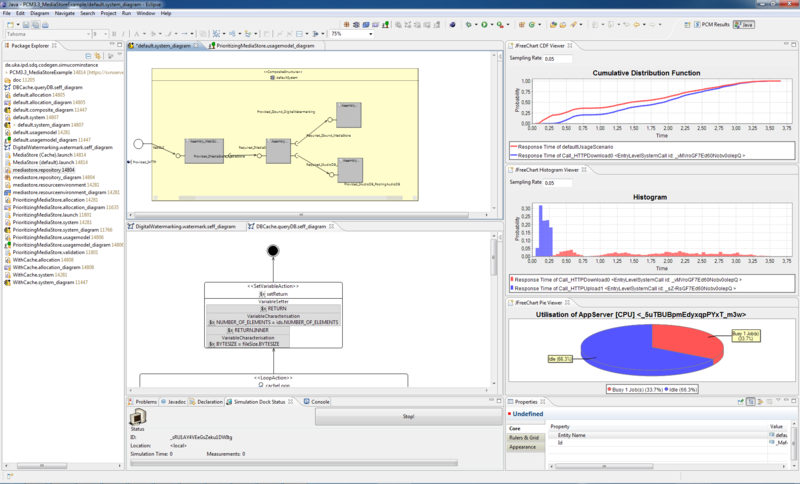
\includegraphics[width=\textwidth]{Bilder/palladio}
				\tiny{Graphical Interface of the Palladio Eclipse Plugin}
			\end{center}

	\end{column}
\end{columns}
\end{frame}

\note[itemize]{
\item Developed at KIT, FZI and University of Paderborn
\item Palladio should be used to evaluate different load balancing strategies or other design decisions (like infrastructure improvements).

\item Architectural Templates: Enables one to efficiently model large systems (E.g. instead of modeling 1000 servers manuelly, model one server and architectural templates duplicates this server 1000 times).
\item SimuLizar: Simulate self adapting systems
}

\section*{Model Computing Jobs}
\begin{frame}
\frametitle{Model Computing Jobs}
\begin{columns}
	\begin{column}{0.45\textwidth}
		\begin{itemize}
		\setlength\itemsep{1em}
			\item Model each kind of computing job with its resource requirements
				\begin{itemize}
					\item CPU \& I/O
					\item Required job slots
					\item Number of events
				\end{itemize}
			\item Model load balancing strategy
				\begin{itemize}
					\item First fit search based on available job slots
					\item Easily modifiable to evaluate new strategies
				\end{itemize}
			\end{itemize}
	\end{column}
	\hfill
	\begin{column}{0.45\textwidth}
		\begin{center}
			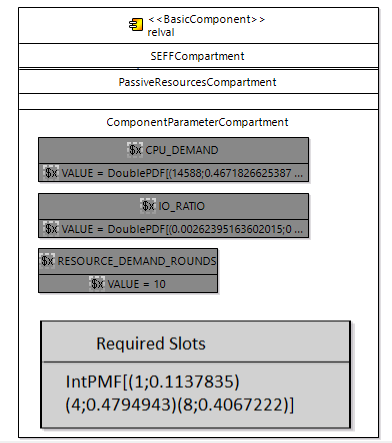
\includegraphics[width=\textwidth]{Bilder/component}
		\end{center}
	\end{column}
\end{columns}
\end{frame}

\note[itemize]{
	\item Different Models of the system are created, on for the resource environment, the assembly (how components work togehter), the usage, the allocation and the component behaviour (e.g. required resources).
	
	\item Required Resources are probability distributions
	\item Jobs block and wait for free slots if not enough job slots are available on working node.
}


\begin{frame}
\frametitle{Model Resource Container}
\begin{columns}
	\begin{column}{0.45\textwidth}
		\begin{itemize}
			\setlength\itemsep{1em}
			\item Model each type of computing node
			\begin{itemize}
				\item Number and processing speed of cores
				\item Processing speed of I/O
				\item Number of job slots
				\item Number of instances of node
			\end{itemize}
			
			\item Model high load on system
			\begin{itemize}
				\item Closed workload
				\item Enough jobs to guarantee that systems never idles
				\item Each job type has configurable share of load
			\end{itemize}
		\end{itemize}
	\end{column}
	\begin{column}{0.45\textwidth}
		\begin{center}
			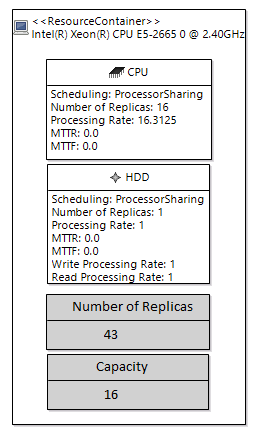
\includegraphics[width=\textwidth]{Bilder/model-container}
		\end{center}
	\end{column}
\end{columns}
\end{frame}

\begin{frame}[c]
    \frametitle{Simulating CMS Jobs at GridKa}
    
    Data Sources:
    \begin{columns}
        \begin{column}{0.45\textwidth}
            \begin{itemize}
                \item Global job monitoring data
                \begin{itemize}
                    \item JobMonitoring, WMArchive job reports \\
                    {\scriptsize from Hadoop analytix cluster with CMSSpark framework (Kuznetsov)}
                    \item Currently extracting CMS jobs at GridKa
                \end{itemize}
                \item Site-specific performance data
                \begin{itemize}
                    \item VO resource share
                    \item Node benchmarks
                \end{itemize}
            \end{itemize}
        \end{column}
        \begin{column}{0.45\textwidth}
            \begin{center}
                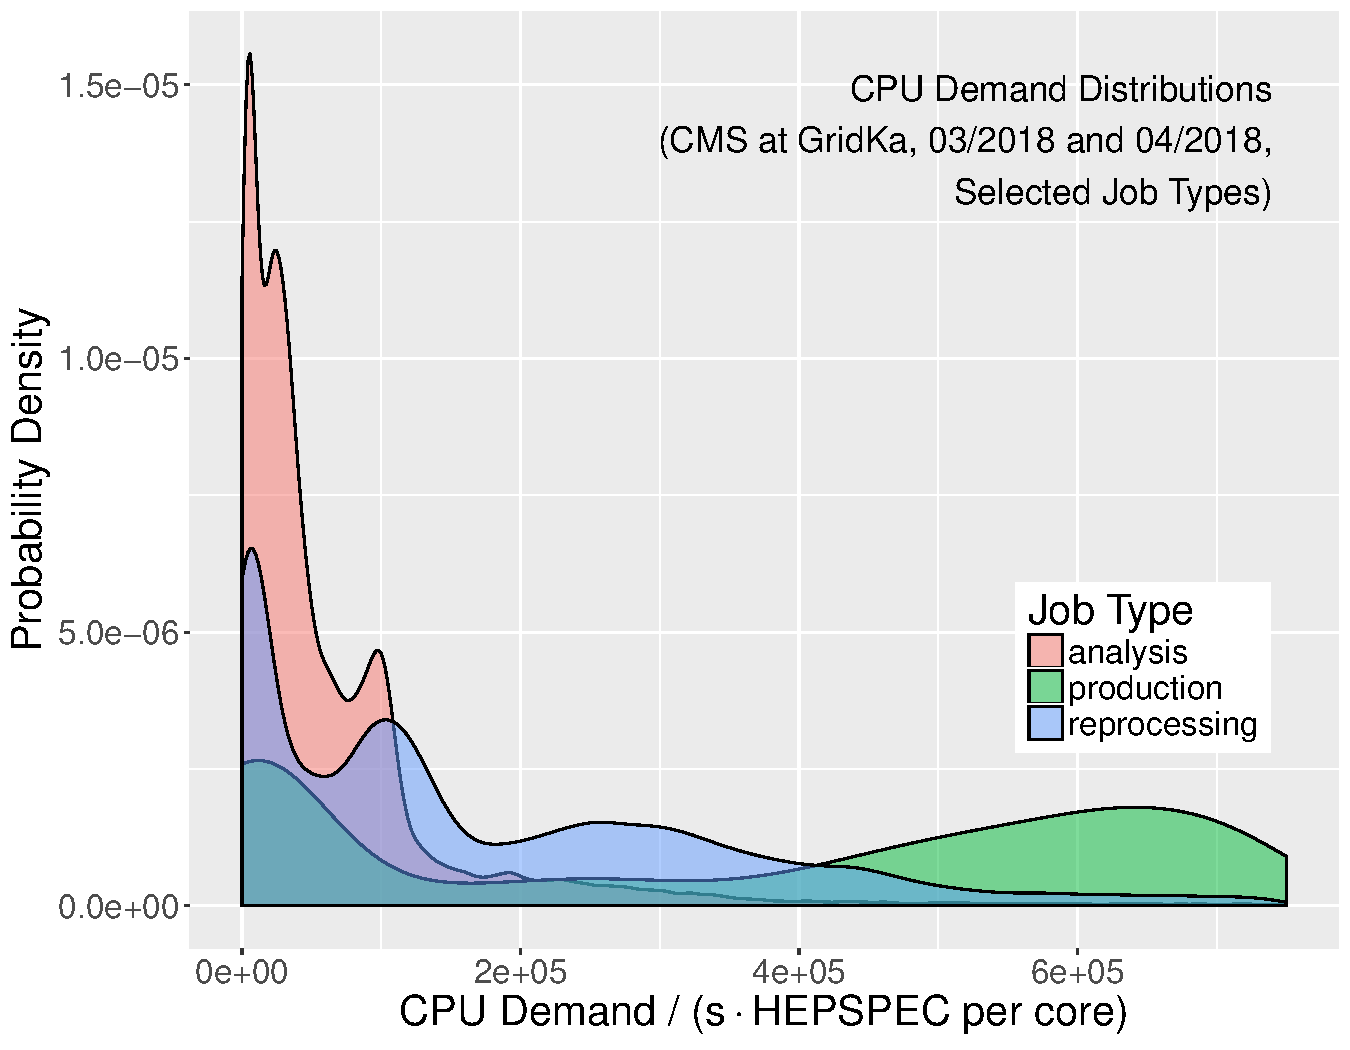
\includegraphics[width=\textwidth]{Bilder/histogram_CPUDemand_all-2018-03to04}
            \end{center}
        \end{column}
    \end{columns}

\end{frame}

\note[itemize]{
    \item Model relies on accurate laod and job resource requirement descriptions
    \item Matching job reports from different subsystems heuristically due to differing monitoring record structures
    \item Simulation model is being generated from extracted model parameters
}

\begin{frame}[c]{Model Calibration Process}
    \begin{columns}
        \begin{column}{0.45\textwidth}
            \setbeamertemplate{enumerate items}[default]
            
            Parameter extraction tool:
            \vspace{1em}
            \begin{enumerate}
                \item \alert{Match} jobs and node performance information
                \item \alert{Group} computing jobs by type and requirements
                \item \alert{Extract} resource demand distributions and load composition
            \end{enumerate}

            
        \end{column}
        \begin{column}{0.45\textwidth}
            \begin{center}
            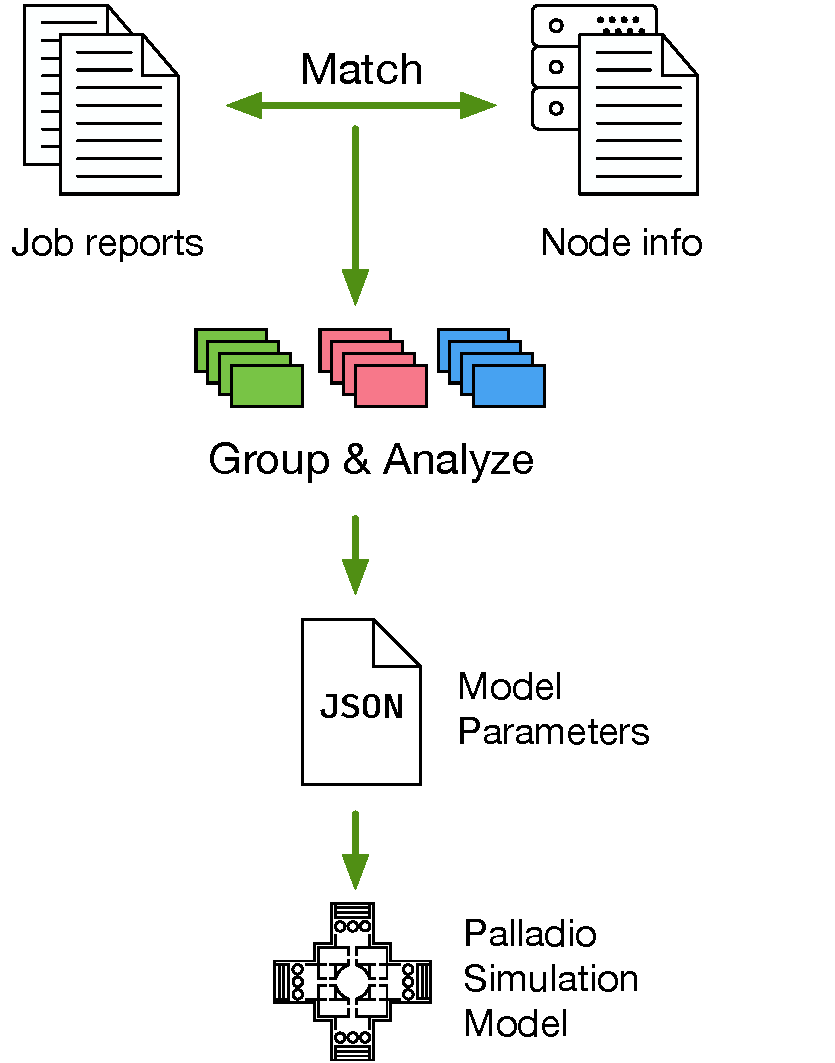
\includegraphics[width=0.8\textwidth]{Bilder/model-parameter-process.pdf}
            \end{center}   
        \end{column}

    \end{columns}
    
\end{frame}



\section*{Validation}
\begin{frame}
\frametitle{Validation}
\begin{columns}
	\begin{column}{0.45\textwidth}
		\begin{center}
		\vspace{-21ex}
		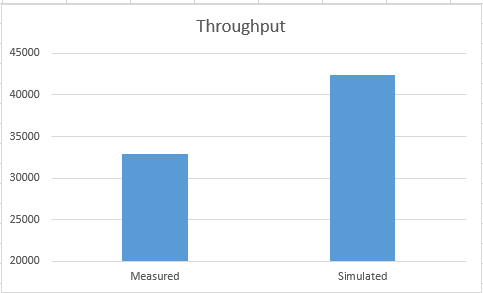
\includegraphics[width=\textwidth]{Bilder/durchsatz}
		\begin{flushleft}
 		{\scriptsize Closed loop validation: Simulation of CMS computing jobs at GridKa for one week. \\
 		Based on measured data from April 2018.}
 		\end{flushleft}
		\end{center}
	\end{column}
	\begin{column}{0.5\textwidth}
		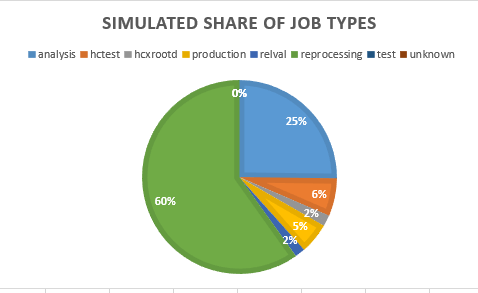
\includegraphics[width=\textwidth]{Bilder/anteil-simuliert}
		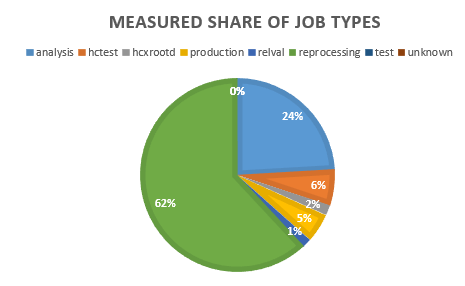
\includegraphics[width=\textwidth]{Bilder/anteil-gemessen}
	\end{column}
\end{columns}
\end{frame}

\begin{frame}
\frametitle{Results}
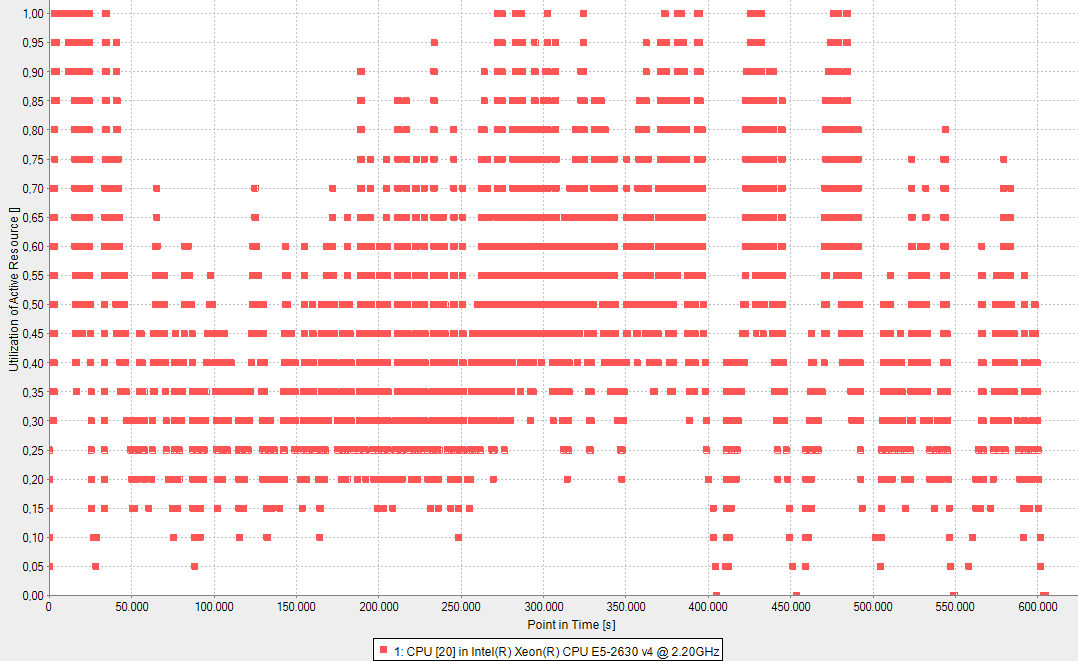
\includegraphics[scale=0.42]{Bilder/utilization}
\end{frame}

\note[itemize]{
	\item Required time to simulate one week is 12min.
	\item Validated with throughput and share of completed jobs per type
	\item Not yet validated with measured utilization.
	\item data from 2018-01tomid02
}

\section*{Outlook}
\begin{frame}
\frametitle{Outlook}
\begin{columns}
	\begin{column}{0.45\textwidth}
		\begin{itemize}
			\item 1
			\item 2
		\end{itemize}
	\end{column}
	\hfill
	\begin{column}{0.45\textwidth}
		\begin{itemize}
			\item 3
			\item 4
		\end{itemize}
	\end{column}
\end{columns}
\end{frame}
\end{document}
